\chapter{Pilot sequence}\label{ch:pilot_sequence}

Mobile technologies have come a long way for exchanging control information and channel dedicated to control information have been designed for most mobile technologies. An important part of the control information is information related to the channel state. This information can help make correct and optimized decisions, given the radio condition that is experienced or expected on a given link. Such information is vital to the optimization of \gls{mimo} transmission due to the selection and configuration of the transmission. From how the symbols should be coded, to how the transmission mode should be configured. The configuration of all parameters related to transmission is in overall terms based on:

\begin{enumerate}
    \item Channel conditions between the transmitter and the receiver (in both uplink and downlink)
    \item Network-wide state
\end{enumerate}

Specific signals (also called reference or pilot signals) are used to sample the channel to obtain information about the channel conditions. Such information is also termed \gls{csi}, and have a long list of use cases in both uplink and downlink transmission.

In this chapter, an introduction to reference signals used in wireless communication will be given. A focus will be on the uplink for one primary reason; \emph{Large quantities of \gls{csi} data is obtained at the base stations which have significant processing capabilities and fewer energy constraints than user terminals \cite{Studer2018}}. A large amount of raw \gls{csi} data from the uplink transmission is a promising place to look for relevant and feasible \gls{dl} solutions as the practicality of computational processing is simplified compared to downlink transmission. In downlink transmission, the processing takes place at the receiver, which in mobile communication systems have several constraints related to energy and computation. This chapter work as an introduction to Chapter \ref{ch:channel_estimation} and \ref{ch:channel_q_learning}. The content of the chapter is organized as follows. An introduction to noticeable literature related to pilot optimization is given with an emphasis on the uplink and relevant problems hereof. Finally, an introduction to the specifics of the pilot signals is given


\section{Introduction}\label{sec:pilot_introduction}

Recently, with the promotion of 5G related solutions, beamforming in \gls{mimo} systems have been hailed as the main driver for pursuing high capacity gains. With the addition of technologies such as \gls{mmwave}, the capacity gains provided by efficient beamforming can offer many Gbps of capacity \cite{Ahmed2018APerspectives}. The task of obtaining updated \gls{csi} is paramount to the efficiency of \gls{mimo} transmission \cite{Lee2012TheInterference, Medard2000TheChannel}. The reference signals used to obtain \gls{csi} are standardized in 4G and 5G in both downlink and uplink. However, as recent studies have shown the increased number of required pilots have a significant impact on the network and the terminals \cite{Elijah2016ASystem}. The use of pilot schemes in both \gls{tdd} and \gls{fdd} systems require significant coordination to avoid interference. As the number of pilots increases across the cellular system, the magnitude of interference is expected to increase - this has recently gained substantial interest in the research community and has been termed \emph{pilot contamination}. 

% To enable the exchange of such information, 2 elements are required. 1) reference signals that are known in order to deduce the channel conditions and 2) a channel on which the information can be exchanged both in downlink and uplink. Such reference signals are also termed \emph{pilot sequences} and is a common practice is communication systems for obtaining insight in the link characteristics. 

% Recently a large amount of studies have notified the research community that a significant number of pilots are used for various reasons. And furthermore, such pilots are the enabler of complex technologies such as \gls{mimo} and effective beamforming. The number of required pilots have increased to improve data transmission speeds and this have a significant impact on both the network and the terminals  

% In case of \gls{tdd}, it can be argued that the link characteristics are reciprocal and thus shared in both uplink and downlink direciton. However, in the case of \gls{fdd} this is not the case. 


The consequences of pilot contamination in \gls{tdd} systems is well described and outlined in the comprehensive work found in \cite{Elijah2016ASystem}. In \gls{tdd} systems, the idea of channel reciprocity is a key feature for minimizing the pilot contamination. The authors in \cite{Elijah2016ASystem} identify the sources of pilot contamination as related to three major factors.

\begin{enumerate}
    \item Non-orthogonal pilot schemes
    \item Hardware impairments
    \item Non-reciprocal transceivers
\end{enumerate}

The sharing of non-orthogonal pilots between cells in a multi-cell system (with frequency reuse) cause inter-cell interference to be the primary source of pilot contamination. The effect of pilot contamination results in imperfect and noisy \gls{csi}, which have a direct impact on the performance of the \gls{mimo} system. (A complete list of relevant literature that studies the effect of imperfect channel knowledge can be found in \cite{Elijah2016ASystem}). However, allocating more pilots to achieve good channel knowledge also has a significant drawback in terms of overhead. In other words, a trade-off exists between pilots needed for obtaining channel knowledge and the result of imperfect channel knowledge. The optimization of pilots is thus two-fold; by increasing the number of pilots, the overhead increases (which have an impact on the \gls{se})—decreasing the amount of pilots results in imperfect channel knowledge also affect \gls{se}.

For \gls{fdd} systems, the problem is amplified furthermore as no reciprocal channel knowledge is available (non-reciprocal transceivers). In short, the problem of pilot contamination for heavily loaded \gls{fdd} systems are equally troublesome, and even furthermore, the channel estimation is required in both downlink and uplink. This has sparked research papers such as \cite{ZirwasKeySystem} that argue if massive \gls{mimo} in \gls{fdd} systems in even a reasonable idea at all. The authors show that a significant overhead (in the range of  $40$ to $50\%$) in \gls{fdd} systems are required for obtaining perfect \gls{csi}. Findings like this furthermore pose the important question: "How to feedback \gls{csi} of downlink channels to the \gls{enb}?". The authors propose the use of a coded \gls{csi} RS pilot scheme that can improve the overall spectral efficiency. Solutions like this are necessary to enable the use of massive \gls{mimo} for downlink in \gls{fdd} systems. But how about uplink? As the authors also state, uplink \gls{csi} is obtained through the use of pilot sequences such as the \gls{srs}. The \gls{srs} sequence in \gls{tdd} systems allow \gls{csi} to be obtained for both uplink and downlink streams due to the reciprocal transceivers. Doing so, effectively means the overhead can be significantly reduced as pilots are only required transmitted in the uplink direction - enabling the cumbersome process of channel estimation to be performed at the \gls{enb}. 

In summary, the problem and consequence of pilot contamination are complex and uncertain. On the one hand, the overhead required for \gls{fdd} systems might be a bottleneck that means the unfeasible implementation of massive \gls{mimo} solutions. On the other hand, \gls{tdd} systems require extensive coordination for uplink pilot schemes to avoid interference. The successful application of Deep Learning demands data that is feasible to obtain. For now, and as mentioned earlier, this is assumed present at the base station. The same quantity of information is in practice available at the terminals. However, the cost associated with processing the \gls{csi} data at the terminals might outweigh the benefits of having such a solution. For such reason, this limits, the initial task of applying Deep Learning to related problems in uplink, e.g. where the data is available at the base station. Before conveying and arguing why Deep Learning can offer a novel solution, one must first study existing solutions available in the literature. In particular, a few research papers provide new solutions to complicated problems of improving the much-needed pilots. The task remains the same, improve channel estimation accuracy given \gls{csi} data using sparse pilot sequences. If the pilot sequences can be scattered and highly adaptive, the overhead of the needed pilots can, in turn, be reduced to combat the defined pilot contamination. 

\subsection{Noticable litterature}
As outlined in Section \ref{sec:pilot_introduction}, one of the key-issues with pilot contamination is inter-cell interference. In \cite{Galati2017UplinkMIMO} a collection of schemes for uplink \gls{srs} allocations are presented to avoid inter-cell interference. In particular, this consists of coordinating the use of sequences between neighbouring base stations. The authors do an excellent job in presenting relevant metrics for contamination (in terms of interference between pilot sequences), for instance, the trade-off between the available downlink \gls{mimo} throughput and the magnitude of contamination. The authors show the shortcomings of traditional \gls{srs} allocation strategies and present a reuse strategy consisting of segmentation in terms of OFDM symbols, or, e.g. the temporal domain. The reuse strategy is two-fold, either aggressively sharing resources or protecting some resources with the aim of decrease interference from neighbouring cells. A list of related literature along with a summary of the state-of-the-art is given within \cite{Galati2017UplinkMIMO} and reference herein.

The notion of improving channel estimation accuracy is also documented to be a logical approach to reducing pilot contamination. This specifically is presented in work such as \cite{Simko2013AdaptiveSystems} and \cite{Simko2013DesignPatterns}. In short, the authors show that adaptive pilot patterns can optimize channel estimation and thus lowering the number of needed pilots. In \cite{Simko2013AdaptiveSystems} the authors present a diamond-shaped pilot symbol pattern (distributed temporal and spatially) with adaptive parameters that can offer a (up to) $80\%$ gain in a \gls{siso} system and up to $850\%$ in a $4 \times 4$ \gls{mimo} system. By adjusting the pilot symbol patterns based on the fundamental radio characteristics, the channel characteristics can be approximated using the least amount of samples. The results are presented as an upper bound of a constrained capacity evaluation. In \cite{Simko2013DesignPatterns}, the authors discuss the problems related to the core issue of feedback overhead. The authors show that by constraining the adaptive pilot patterns, a wide range of Doppler spreads and delay spreads can be supported, resulting in requiring only 4 bits for feedback. 

% A comphrensive review and survey on hybrid beamforming techniques for 5G solutions can be found in  \cite{Ahmed2018APerspectives}. The authors discuss the importance of \gls{csi} for massive \gls{mimo} communication systems, and furthermore, it comes more important 


% \cite{Muppirisetty2018Location-AidedSystems}


\section{Sounding Reference Signal}\label{sec:srs_sequence_definition}

The \gls{srs} is a term for pilot signals sent in uplink and as defined by \gls{3gpp} for \gls{lte} and \gls{nr} systems. The pilot schemes are detailed in technical documents \cite{36211, 3GPP2020TS15} for \gls{lte} and \gls{lte}-A systems. For \gls{nr} systems \gls{srs} is detailed in the technical documents \cite{38211, 3GPP2020TS15b}. For both systems, the Zadoff-Chu sequence is used for the pilot symbols due to the excellent properties of orthogonality. Secondly, \gls{srs} symbols are always transmitted on the last \gls{ofdm} symbol of the scheduled subframe, if any only if, a transmission comb does not enable additional \gls{ofdm} symbols to be utilized. Finally, the \gls{srs} configuration is determined by the serving cell and can be adjusted to specific requirements. An example of an \gls{srs} pilot sequence can be seen in Fig. \ref{fig:srs_pilot_example}.

\begin{figure}
    \centering
    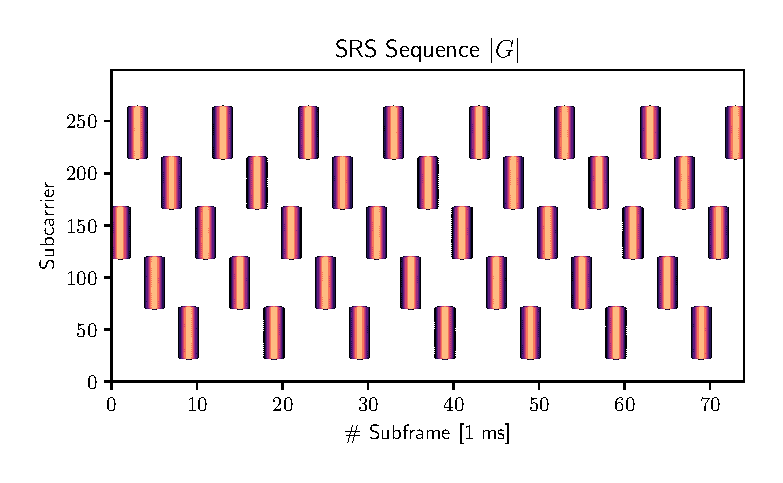
\includegraphics{chapters/part_uplink/figures/srs_pilot_example.eps}
    \caption{An example of an \gls{srs} sequence with \texttt{srs-FreqHopping} enabled over $300$ subcarriers.}
    \label{fig:srs_pilot_example}
\end{figure}


This section will attempt to detail the necessary details from the standardization documents required for posing and visualizing the nature of the \gls{srs} pilot sequence. The section will furthermore outline the difference between \gls{lte} and \gls{nr} standardization in an attempt to structure and detail trends for future standardization documents. 

\subsection{Configuration parameters}
The documents \cite{36211,3GPP2020TS15} (36211 and 36213) contains the majority of the information related to the standardization of the \gls{srs} sequence for \gls{lte} systems. The information is extremely comprehensive and considers all combinations of configurations in \gls{lte} systems. In brief terms, \gls{srs} considers 2 trigger types; Periodic or a single pilot sequence, also called \emph{type 0}. Usually, the configuration of \emph{type 0} is determined by higher-layer parameters. Asynchronous \emph{type 1} is triggered by the \gls{dci}. For each trigger type, depending on the mode of operation, e.g. \gls{tdd} or \gls{fdd} a difference in not only available configurations but also available parameters can be found. In short, it is a set of complicated and complex configuration interactions. Furthermore, each \gls{ue} may configure \gls{srs} on each serving cell. A large number of parameters are essential for the configuration of the \gls{srs} sequence; however, some are essential for configuring fundamental characteristics such as bandwidth and periodicity. These are given in Table \ref{tab:srs_config_param}.

% Please add the following required packages to your document preamble:
% \usepackage{booktabs}
\begin{table*}[]
\begin{tabular}{@{}llp{8cm}@{}}
\toprule
Parameter            & Notation  & Description                                                           \\ \midrule
-                    & $n_{RRC}$    & Starting physical resource block (determined by \texttt{freqDomainPosition})   \\
srs-ConfigIndex      & $I_{SRS}$    & Table lookup index for periodicty $T_{SRS}$ and subframe offset $T_{offset}$   \\
srs-Bandwidth        & $B_{SRS}$    & Bandwidth of the SRS sequence                                        \\
srs-SubframeOffset   & $T_{offset}$ & Subframe offset configuration                                         \\
srs-SubframePeriod   & $T_{SRS}$    & Periodicity configuration                                             \\
srs-HoppingBandwidth & $b_{hop}$    & Bandwidth of frequency hopping                                        \\
srs-BandwidthConfig  & $C_{SRS}$    & Cell-specific bandwidth parameter                                     \\ \bottomrule
\end{tabular}
\vspace{1em}
\caption{Essential \gls{srs} configuration parameters}\label{tab:srs_config_param}
\end{table*}

The remainder of the needed parameters for constructing the \gls{srs} sequence are given by various tables in \cite{36211,3GPP2020TS15}. For instance, having an uplink bandwidth of $40$ to $60$ resource blocks refers to Table 5.5.3.2-2 in 36.211. Supplied by the table, the configuration of cell-specific bandwidth $C_{SRS}$, and the bandwidth of the \gls{ue} $B_{SRS}$ - the length of the resulting Zadoff-Chu sequence is calculated. The $I_{SRS}$ parameters refer to Table 5.5.3.3-1 in 36.211, that determines the periodicity and the transmission offset.


\paragraph{NR}
A set of documents details the configuration of \gls{srs} sequences in \gls{nr} systems \cite{38211, 3GPP2020TS15b} (38211 and 38213). A similar use of parameters and interactions can be observed from the technical documents. Most noticeably is the simplification of the table lookups required for determining the length of the resulting \gls{srs} sequence. This also means that $C_{SRS}$ assumes integers from $[0,.., 63]$ instead of $[0,..,7]$ split over 4 different tables. For \gls{nr}, Table 6.4.1.4.3-1 in 38211 contains the much needed information required for the \gls{srs} bandwidth configuration.
